\subsection{Crystal structure}

There are different ways a solid could arrange itself in order to fill a given volume and minimize the overall energy of the structure. One of the densest is the face-centered cubic (FCC) structure of for instance NaCl. Assuming a hard sphere model of atoms, the FCC has together with the hexagonal close packed (HCP) the theoretically highest density of any structure. The unit cell of FCC is cubic with volume $ V_{unitCell} = a^3 $ made up by a basis of 4 atoms. These are in positions $ a(0,0,0), \ a(0,0,\frac{1}{2}),\ a(0,\frac{1}{2}, 0)   $ and $ a(\frac{1}{2}, 0,0) $. Due to symmetry, each of these atoms are repeated throughout the structure, as illustrated in figure \ref{fig:fcc}. The corner atoms are  repetitions of the $ a(0,0,0)$ position, and each of these atoms are shared by 8 neighbouring cells. For the side atoms, they are shared only by two unit cells, giving at total of $ 6\cdot \frac{1}{2}=3 $ side atoms per unit cell and $ 8\cdot  \frac{1}{8}$ corner atoms in the unit cell. The density of a unit cell size given in lengths of Angstrom, the density of a FCC cell  is $\rho=  \frac{4}{a^3} \text{\AA}^{-3}$. 

\begin{figure}[H]
	\centering
	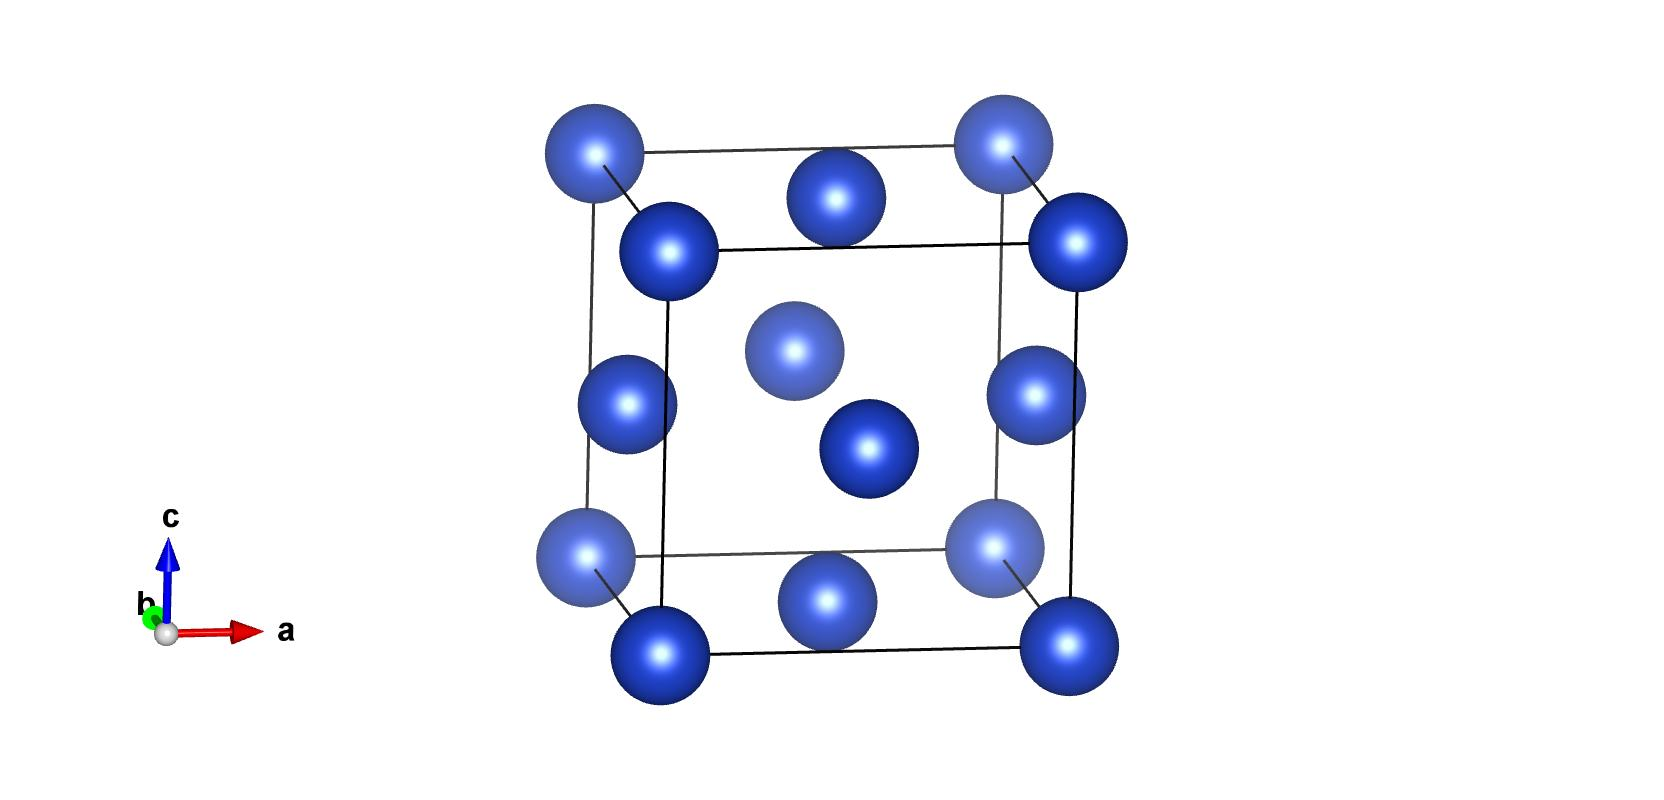
\includegraphics[width=0.7\linewidth]{../figures/fcc.jpg}
	\caption{Illustration of a fcc structure. Although there are 14 atoms in this figure, the unit cell is made up of 4 atoms. The rest of the atoms appear because of translation symmetry. Illustration is created by the VESTA software \cite{VESTA}}
	\label{fig:fcc}
\end{figure}

\subsection{Lennard Jones potential \label{sec:LJ}}

A very popular potential used in MD-simulations is the Lennard Jones potential, given in equation \ref{eq:LJ}. It describes the potential energy as a function of distance between two objects i and j, $ r_{ij} $. 

\begin{equation}\label{eq:LJ}
	U(r_{ij}) = 4\epsilon \left[	\left(\frac{\sigma}{r_{ij}}	\right)^{12}		- \left(\frac{\sigma}{r_{ij}}	\right)^{6}				\right]\\
\end{equation}




Through the relation $ 	F (\textbf{r} = -\nabla U(\textbf{r}) $, it is possible to determine the forces experienced by each atom by every other atom, simply as a function of the distance $ r_{ij} $ and relative position between two atoms. The distance $ r_{ij} $ is defined as  $ r_{ij}  = \abs{\textbf{r}_{ij}} = \abs{\textbf{r}_i - \textbf{r}_j} 	 $. 

\begin{align}
		F_{ij}^x =& - \pdv{U}{r_{ij}} \pdv{r_{ij}}{x_{ij}} = - \pdv{U}{r_{ij}} \frac{x_{ij}}{r_{ij}}	\\	
		 F_x(r_{ij}) =& 24 \epsilon \left[		2	\left(\frac{\sigma}{r_{ij}}	\right)^{12}		- \left(\frac{\sigma}{r_{ij}}	\right)^{6}				\right] \frac{x_{ij}}{r_{ij}^2} \label{eq:Fx}
\end{align}

By generalising equation \ref{eq:Fx} to a three dimensional space one gets a general expression of the force between two atoms i and j: 
\begin{equation}\label{eq:F}
		  \textbf{F}(r_{ij}) = 24 \epsilon \left[		2	\left(\frac{\sigma}{r_{ij}}	\right)^{12}		- \left(\frac{\sigma}{r_{ij}}	\right)^{6}				\right] \frac{\textbf{r}_{ij}}{r_{ij}^2}
\end{equation}

In figure \ref{fig:lj} both the potentate and force is illustrated, clearly showing that the repulsion from the $ \left(	\frac{\sigma}{r_{ij}}\right)^{12} $ term is very strong at low values of $ r_{ij}$. For larger $ r_{ij} $ both terms quickly goes towards 0. However, the potential display a minimum before it goes towards zero, determined by $ \sigma $. For distances smaller than $ \sigma $, the force is positive and thus repulsive and for $ r_{ij} >\sigma $ is shows attractive properties. The forces is never truly 0 before $ r_{ij}  = \infty$. but for most practical purposes it is mainly the distances $ r_{ij} \in [0,10] $ that contribute to the total force on each atom. 


\begin{figure}[H]
	\centering
	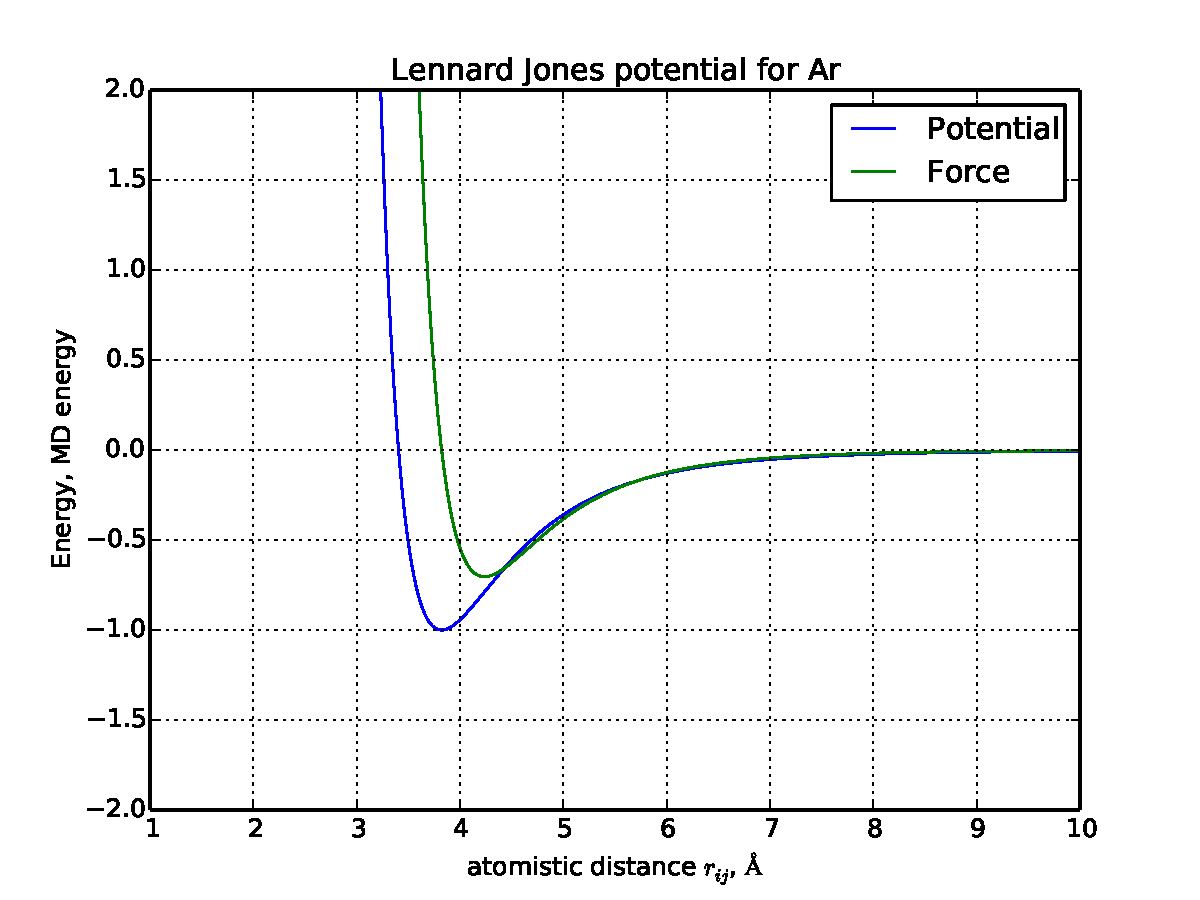
\includegraphics[width=0.7\linewidth]{../figures/LJ}
	\caption{Illustration of the Lennard Jones potential. See section \ref{sec:units} for definition of the MD units}
	\label{fig:lj}
\end{figure}


Atom $ i $ experience a total force of $ F(\textbf{r}_i) =  \sum\limits_{j\neq i}   \textbf{F}(r_{ij})$. Each interaction is only necessary to compute once, as $ \textbf{r}_{ij}  = - \textbf{r}_{ji} $. However, it is necessary to update the force on each atom, according to Newtons third law. Equivalently, the total potential is given as $ U_{tot} =  \sum\limits_{i} \sum\limits_{j>i} 	U(\textbf{r}_{ij}) $. 



\subsection{The microcanonical ensemble}
This subsection is based on M. Jensen \cite{Jensen}. 

In statistical physics, the microcanonical ensemble is a system with constant volume, particles and total energy. This means that it is an isolated system which does not exchange energy or particles  with the surroundings, but are allowed to vary the pressure and temperature. As with any ensemble in statistical physics, the equilibrium is reached when the system is near the most probable state. As Maxwell-Boltzmann statistics governs the probability of each microstate, the equilibrium is dependent on both temperature and energy of the state. In the microcanonical ensemble, temperature $ T $ and pressure $ P $ are defined through the number of possible microstates $ \Omega $ as:

\begin{align}
S &= k_B\log \Omega\\
\frac{1}{T} &= \left(  	\pdv{S}{E}	\right)_{N,V} \label{eq:T}\\
p &= k_BT \left(	\pdv{\log\Omega	}{V}	\right)_{N,E} \label{eq:P}
\end{align}

At equilibrium, every microstate has the same total energy. This leads to  the equipartition theorem, stating that it every microstate is equally probable and will be at some point occupied. One example of a microstate not conforming to this is the microstate where all the atoms are located in a sphere of very low radius - giving an infinite potential, see the discussion about the Lennard Jones potential in section \ref{sec:LJ}. 

Through the equipartition theorem, the following relationship for a 3 dimensional system arises between the total kinetic energy of the system and the temperature:

\begin{equation}\label{eq:equipartition}
E_K = \frac{3	}{2}Nk_BT
\end{equation}

As the temperature at equilibrium is related to the kinetic energy, any system system resembling a real system needs to have kinetic energy >0. The pure lattice points of the FCC lattice has a high degree of symmetry and the force on each atom would for a infinite lattice cancel out to 0. It is therefore necessary to include an initial velocity in order to model the structure at different temperatures, due to the equipartition relation in equation \ref{eq:equipartition}. As the total kinetic energy does not provide any information about the velocity of each atom, the probability distribution utilized for the microcanonical ensemble is a good way to initialize the system to progress into a new, random microstate in the next time step. 

By including an initial velocity, there is no guaranty that the total momentum $ p = \sum\limits_{i}^{N} m_i\textbf{v}_i $ is zero. In order to keep the system fixed in space, the total momentum need to be set to zero, by reducing the momentum of each atom by $ m_iv_i - \frac{p}{N}$. 

\subsubsection{Diffusion and phase transition}
Diffusion is a property of any microcanonical ensemble, characterized by the diffusivity $ D $. Through the Einstein relation
\begin{equation}\label{eq:Einstein}
\langle r^2(t) \rangle = 6Dt
\end{equation}

the diffusivity is related to the mean square displacement $ r_i^2(t) = \abs{r_i(t) - r_i(o)}^2 $. The diffusivity is approximately 10$^{-5}$ cm$^2$/s in liquids and 10$^{-9}$ cm$^2$/s for in solids, for example hydrogen in iron \cite{wiki_diff}. 

\subsection{Density}

The density of argon is 0.001784 g/cm$^3$ at STP when gas and 1.3954 g/cm$^3$ at the boiling point when liquid \cite{argon}. Table \ref{tab:density} compare these numbers with the system in this project. Experimentally argon has a melting temperature at 84 K and a boiling temperature at 87 K at 1 atm \cite{argon}. The densities implies that even though argon has only 3 degrees in liquid the state at 1 atm, the density of our system is too high for it to transit to gas. 

\begin{table}[H]\caption{This table list the calculation of the density and compare the density of liquid argon, argon gas and our system. We used the molar mass of argon, 39.948 g/mol \cite{argon}.}\label{tab:density}
\center
\renewcommand{\arraystretch}{2}
\begin{tabular}{r|lr}
 &calculation:&  density $\left[ \frac{\text{\# of atoms}}{\text{cm}^3} \right]$:\\ \hline
Gas:& $\frac{0.001784 \text{ g/cm}^3 }{39.948 \text{ g/mol}}$ = 4.46580$\cdot 10^{-5}$ $\frac{\text{mol}}{\text{cm}^3}$ = & 2.6893$\cdot$ 10$^{19}$ \\
Liquid:& $\frac{1.3954 \text{ g/cm}^3 }{39.948 \text{ g/mol}}$ = 0.0349304 $\frac{\text{mol}}{\text{cm}^3}$ =& 2.10350$\cdot$ 10$^{22}$\\
This system:& $\frac{4}{a^3} = \frac{4}{5.26^3}$ = 0.027485 $\frac{\text{\# of atoms}}{\text{Å}^3}$ =& 2.74854 $\cdot$ 10$^{22}$\\
\end{tabular}
\end{table}